% Options for packages loaded elsewhere
\PassOptionsToPackage{unicode}{hyperref}
\PassOptionsToPackage{hyphens}{url}
%
\documentclass[
  12pt,
]{article}
\usepackage{amsmath,amssymb}
\usepackage{lmodern}
\usepackage{ifxetex,ifluatex}
\ifnum 0\ifxetex 1\fi\ifluatex 1\fi=0 % if pdftex
  \usepackage[T1]{fontenc}
  \usepackage[utf8]{inputenc}
  \usepackage{textcomp} % provide euro and other symbols
\else % if luatex or xetex
  \usepackage{unicode-math}
  \defaultfontfeatures{Scale=MatchLowercase}
  \defaultfontfeatures[\rmfamily]{Ligatures=TeX,Scale=1}
\fi
% Use upquote if available, for straight quotes in verbatim environments
\IfFileExists{upquote.sty}{\usepackage{upquote}}{}
\IfFileExists{microtype.sty}{% use microtype if available
  \usepackage[]{microtype}
  \UseMicrotypeSet[protrusion]{basicmath} % disable protrusion for tt fonts
}{}
\makeatletter
\@ifundefined{KOMAClassName}{% if non-KOMA class
  \IfFileExists{parskip.sty}{%
    \usepackage{parskip}
  }{% else
    \setlength{\parindent}{0pt}
    \setlength{\parskip}{6pt plus 2pt minus 1pt}}
}{% if KOMA class
  \KOMAoptions{parskip=half}}
\makeatother
\usepackage{xcolor}
\IfFileExists{xurl.sty}{\usepackage{xurl}}{} % add URL line breaks if available
\IfFileExists{bookmark.sty}{\usepackage{bookmark}}{\usepackage{hyperref}}
\hypersetup{
  pdftitle={ADA2: Class 11, Chs 05 and 07, writing and plotting model equations},
  pdfauthor={Name Here},
  hidelinks,
  pdfcreator={LaTeX via pandoc}}
\urlstyle{same} % disable monospaced font for URLs
\usepackage[margin=0.25in]{geometry}
\usepackage{color}
\usepackage{fancyvrb}
\newcommand{\VerbBar}{|}
\newcommand{\VERB}{\Verb[commandchars=\\\{\}]}
\DefineVerbatimEnvironment{Highlighting}{Verbatim}{commandchars=\\\{\}}
% Add ',fontsize=\small' for more characters per line
\usepackage{framed}
\definecolor{shadecolor}{RGB}{248,248,248}
\newenvironment{Shaded}{\begin{snugshade}}{\end{snugshade}}
\newcommand{\AlertTok}[1]{\textcolor[rgb]{0.94,0.16,0.16}{#1}}
\newcommand{\AnnotationTok}[1]{\textcolor[rgb]{0.56,0.35,0.01}{\textbf{\textit{#1}}}}
\newcommand{\AttributeTok}[1]{\textcolor[rgb]{0.77,0.63,0.00}{#1}}
\newcommand{\BaseNTok}[1]{\textcolor[rgb]{0.00,0.00,0.81}{#1}}
\newcommand{\BuiltInTok}[1]{#1}
\newcommand{\CharTok}[1]{\textcolor[rgb]{0.31,0.60,0.02}{#1}}
\newcommand{\CommentTok}[1]{\textcolor[rgb]{0.56,0.35,0.01}{\textit{#1}}}
\newcommand{\CommentVarTok}[1]{\textcolor[rgb]{0.56,0.35,0.01}{\textbf{\textit{#1}}}}
\newcommand{\ConstantTok}[1]{\textcolor[rgb]{0.00,0.00,0.00}{#1}}
\newcommand{\ControlFlowTok}[1]{\textcolor[rgb]{0.13,0.29,0.53}{\textbf{#1}}}
\newcommand{\DataTypeTok}[1]{\textcolor[rgb]{0.13,0.29,0.53}{#1}}
\newcommand{\DecValTok}[1]{\textcolor[rgb]{0.00,0.00,0.81}{#1}}
\newcommand{\DocumentationTok}[1]{\textcolor[rgb]{0.56,0.35,0.01}{\textbf{\textit{#1}}}}
\newcommand{\ErrorTok}[1]{\textcolor[rgb]{0.64,0.00,0.00}{\textbf{#1}}}
\newcommand{\ExtensionTok}[1]{#1}
\newcommand{\FloatTok}[1]{\textcolor[rgb]{0.00,0.00,0.81}{#1}}
\newcommand{\FunctionTok}[1]{\textcolor[rgb]{0.00,0.00,0.00}{#1}}
\newcommand{\ImportTok}[1]{#1}
\newcommand{\InformationTok}[1]{\textcolor[rgb]{0.56,0.35,0.01}{\textbf{\textit{#1}}}}
\newcommand{\KeywordTok}[1]{\textcolor[rgb]{0.13,0.29,0.53}{\textbf{#1}}}
\newcommand{\NormalTok}[1]{#1}
\newcommand{\OperatorTok}[1]{\textcolor[rgb]{0.81,0.36,0.00}{\textbf{#1}}}
\newcommand{\OtherTok}[1]{\textcolor[rgb]{0.56,0.35,0.01}{#1}}
\newcommand{\PreprocessorTok}[1]{\textcolor[rgb]{0.56,0.35,0.01}{\textit{#1}}}
\newcommand{\RegionMarkerTok}[1]{#1}
\newcommand{\SpecialCharTok}[1]{\textcolor[rgb]{0.00,0.00,0.00}{#1}}
\newcommand{\SpecialStringTok}[1]{\textcolor[rgb]{0.31,0.60,0.02}{#1}}
\newcommand{\StringTok}[1]{\textcolor[rgb]{0.31,0.60,0.02}{#1}}
\newcommand{\VariableTok}[1]{\textcolor[rgb]{0.00,0.00,0.00}{#1}}
\newcommand{\VerbatimStringTok}[1]{\textcolor[rgb]{0.31,0.60,0.02}{#1}}
\newcommand{\WarningTok}[1]{\textcolor[rgb]{0.56,0.35,0.01}{\textbf{\textit{#1}}}}
\usepackage{longtable,booktabs,array}
\usepackage{calc} % for calculating minipage widths
% Correct order of tables after \paragraph or \subparagraph
\usepackage{etoolbox}
\makeatletter
\patchcmd\longtable{\par}{\if@noskipsec\mbox{}\fi\par}{}{}
\makeatother
% Allow footnotes in longtable head/foot
\IfFileExists{footnotehyper.sty}{\usepackage{footnotehyper}}{\usepackage{footnote}}
\makesavenoteenv{longtable}
\usepackage{graphicx}
\makeatletter
\def\maxwidth{\ifdim\Gin@nat@width>\linewidth\linewidth\else\Gin@nat@width\fi}
\def\maxheight{\ifdim\Gin@nat@height>\textheight\textheight\else\Gin@nat@height\fi}
\makeatother
% Scale images if necessary, so that they will not overflow the page
% margins by default, and it is still possible to overwrite the defaults
% using explicit options in \includegraphics[width, height, ...]{}
\setkeys{Gin}{width=\maxwidth,height=\maxheight,keepaspectratio}
% Set default figure placement to htbp
\makeatletter
\def\fps@figure{htbp}
\makeatother
\setlength{\emergencystretch}{3em} % prevent overfull lines
\providecommand{\tightlist}{%
  \setlength{\itemsep}{0pt}\setlength{\parskip}{0pt}}
\setcounter{secnumdepth}{-\maxdimen} % remove section numbering
\usepackage{booktabs}
\usepackage{longtable}
\usepackage{array}
\usepackage{multirow}
\usepackage{wrapfig}
\usepackage{float}
\usepackage{colortbl}
\usepackage{pdflscape}
\usepackage{tabu}
\usepackage{threeparttable}
\usepackage{threeparttablex}
\usepackage[normalem]{ulem}
\usepackage{makecell}
\usepackage{xcolor}
\ifluatex
  \usepackage{selnolig}  % disable illegal ligatures
\fi

\title{ADA2: Class 11, Chs 05 and 07, writing and plotting model
equations}
\author{Name Here}
\date{February 25, 2022}

\begin{document}
\maketitle

\textbf{This assignment is to be printed and hand-written.}

In my opinion, some of the most important skills in modeling are:

\begin{itemize}
\tightlist
\item
  writing down a model using indicator variables,
\item
  interpretting model coefficients,
\item
  solving for the predicted value for any combination of predictors, and
\item
  plotting the fitted model.
\end{itemize}

This assignment applies these skills to two-way factor models (ADA2
Chapter 5) and ANCOVA models with one factor and one continuous
predictor (ADA2 Chapter 7).

\hypertarget{two-way-main-effect-model-kangaroo-crest-width}{%
\section{1. Two-way main-effect model: Kangaroo crest
width}\label{two-way-main-effect-model-kangaroo-crest-width}}

Recall these data, results, and the model from Week 05.

\begin{Shaded}
\begin{Highlighting}[]
\FunctionTok{library}\NormalTok{(erikmisc)}
\FunctionTok{library}\NormalTok{(tidyverse)}

\NormalTok{kang }\OtherTok{\textless{}{-}}
  \FunctionTok{read\_csv}\NormalTok{(}
    \StringTok{"\textasciitilde{}/Dropbox/3\_Education/Courses/stat\_528\_ada2/ADA2\_CL\_09\_kang.csv"}
\NormalTok{  , }\AttributeTok{na =} \FunctionTok{c}\NormalTok{(}\StringTok{""}\NormalTok{, }\StringTok{"."}\NormalTok{)}
\NormalTok{  ) }\SpecialCharTok{\%\textgreater{}\%}
  \CommentTok{\# subset only our columns of interest}
  \FunctionTok{select}\NormalTok{(}
\NormalTok{    sex, species, cw}
\NormalTok{  ) }\SpecialCharTok{\%\textgreater{}\%}
  \CommentTok{\# make dose a factor variable and label the levels}
  \FunctionTok{mutate}\NormalTok{(}
    \AttributeTok{sex     =} \FunctionTok{factor}\NormalTok{(sex    , }\AttributeTok{labels =} \FunctionTok{c}\NormalTok{(}\StringTok{"M"}\NormalTok{,}\StringTok{"F"}\NormalTok{))}
\NormalTok{  , }\AttributeTok{species =} \FunctionTok{factor}\NormalTok{(species, }\AttributeTok{labels =} \FunctionTok{c}\NormalTok{(}\StringTok{"Mg"}\NormalTok{, }\StringTok{"Mfm"}\NormalTok{, }\StringTok{"Mff"}\NormalTok{))}
\NormalTok{  )}

\FunctionTok{str}\NormalTok{(kang)}
\end{Highlighting}
\end{Shaded}

\begin{verbatim}
tibble [148 x 3] (S3: tbl_df/tbl/data.frame)
 $ sex    : Factor w/ 2 levels "M","F": 1 1 1 1 1 1 1 1 1 1 ...
 $ species: Factor w/ 3 levels "Mg","Mfm","Mff": 1 1 1 1 1 1 1 1 1 1 ...
 $ cw     : num [1:148] 153 141 144 116 120 188 149 128 151 103 ...
\end{verbatim}

\begin{tabular}{l|l|r}
\hline
sex & species & m\\
\hline
M & Mg & 103.0800\\
\hline
M & Mfm & 101.6522\\
\hline
M & Mff & 127.8000\\
\hline
F & Mg & 117.1600\\
\hline
F & Mfm & 128.4800\\
\hline
F & Mff & 161.0000\\
\hline
\end{tabular}

\begin{center}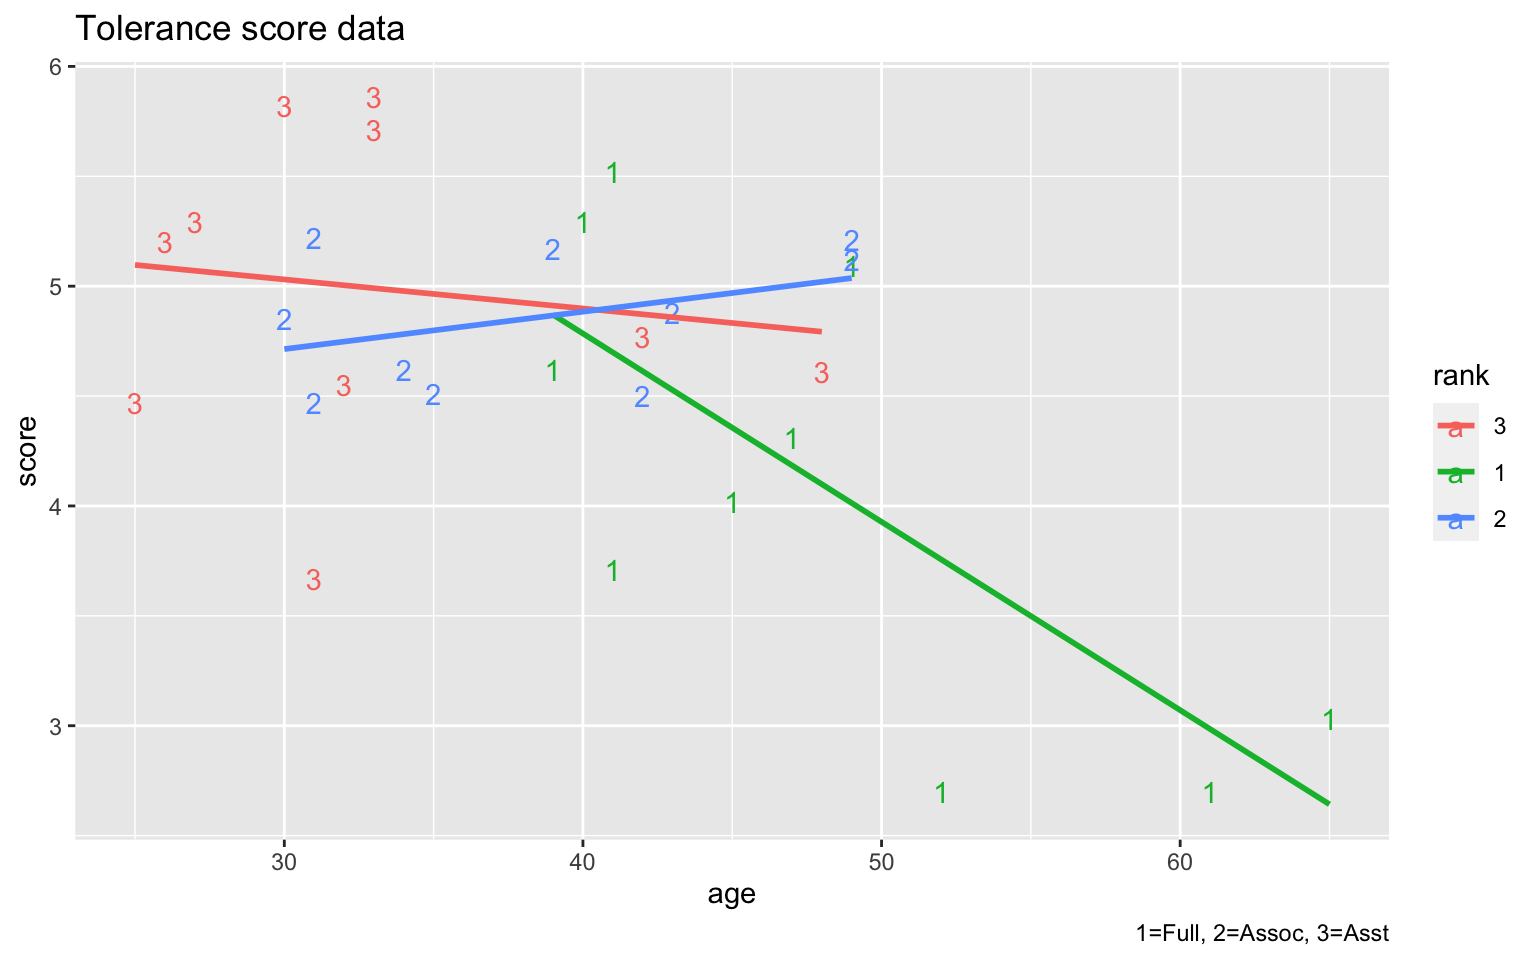
\includegraphics{ADA2_CL_11_ModelEquationsPlots_files/figure-latex/unnamed-chunk-3-1} \end{center}

\begin{Shaded}
\begin{Highlighting}[]
\NormalTok{lm\_cw\_x\_s }\OtherTok{\textless{}{-}}
  \FunctionTok{lm}\NormalTok{(}
\NormalTok{    cw }\SpecialCharTok{\textasciitilde{}}\NormalTok{ sex }\SpecialCharTok{+}\NormalTok{ species}
\NormalTok{  , }\AttributeTok{data =}\NormalTok{ kang}
\NormalTok{  )}
\CommentTok{\# parameter estimate table}
\FunctionTok{summary}\NormalTok{(lm\_cw\_x\_s)}
\end{Highlighting}
\end{Shaded}

\begin{verbatim}
Call:
lm(formula = cw ~ sex + species, data = kang)

Residuals:
    Min      1Q  Median      3Q     Max 
-94.456 -19.746   1.553  23.478  90.216 

Coefficients:
            Estimate Std. Error t value Pr(>|t|)    
(Intercept)   97.784      6.039  16.193  < 2e-16 ***
sexF          24.673      6.070   4.064 7.89e-05 ***
speciesMfm     4.991      7.460   0.669    0.505    
speciesMff    34.280      7.383   4.643 7.66e-06 ***
---
Signif. codes:  0 '***' 0.001 '**' 0.01 '*' 0.05 '.' 0.1 ' ' 1

Residual standard error: 36.91 on 144 degrees of freedom
Multiple R-squared:  0.2229,    Adjusted R-squared:  0.2067 
F-statistic: 13.77 on 3 and 144 DF,  p-value: 6.057e-08
\end{verbatim}

\hypertarget{p-write-the-fitted-model-equation.}{%
\subsection{\texorpdfstring{\textbf{(3 p)} Write the fitted model
equation.}{(3 p) Write the fitted model equation.}}\label{p-write-the-fitted-model-equation.}}

Use the parameter estimate table above to write out the fitted model
equation. Use indicator function notation for categorical variables.
First determine what each sex and species number is. The equation looks
like: \(\hat{y} = [\text{terms}]\).

\hypertarget{solution}{%
\subsubsection{Solution}\label{solution}}

\[ 
\widehat{cw} = 97.8 
+ 24.7 * I(\text{sex = F}) 
+ 5.0 * I(\text{sp. = Mfm}) 
+ 34.3 * I(\text{sp. = Mff})
\]

\hypertarget{p-separate-model-equations.}{%
\subsection{\texorpdfstring{\textbf{(2 p)} Separate model
equations.}{(2 p) Separate model equations.}}\label{p-separate-model-equations.}}

For each combination of species and sex, write the model.

\hypertarget{solution-1}{%
\subsubsection{Solution}\label{solution-1}}

\begin{longtable}[]{@{}lll@{}}
\toprule
Sex & Species & Fitted Model \\
\midrule
\endhead
M & Mg & \(\hat{y}= 97.8\) \\
\textbackslash{} & & \\
M & Mfm & \(\hat{y}= 97.8 + 5.0 = 102.8\) \\
\textbackslash{} & & \\
M & Mff & \(\hat{y}= 97.8 + 34.3 = 132.1\) \\
\textbackslash{} & & \\
F & Mg & \$\hat{y}= 97.8 + 24.7 = 122.5 \$ \\
\textbackslash{} & & \\
F & Mfm & \(\hat{y}= 97.8 + 24.7 + 5.0 = 127.5\) \\
\textbackslash{} & & \\
F & Mff & \(\hat{y}= 97.8 + 24.7 + 34.3 = 156.8\) \\
\bottomrule
\end{longtable}

\hypertarget{p-plot-the-observed-and-fitted-values.}{%
\subsection{\texorpdfstring{\textbf{(0 p)} Plot the observed and fitted
values.}{(0 p) Plot the observed and fitted values.}}\label{p-plot-the-observed-and-fitted-values.}}

Use symbols/colors/labels to distinguish between the observed and
predicted values and clearly identify the species/sex combinations. Use
the minimum about of labeling to make it clear.

\hypertarget{solution-2}{%
\subsubsection{Solution}\label{solution-2}}

COVID-19 Year, no hand plotting :(

\begin{center}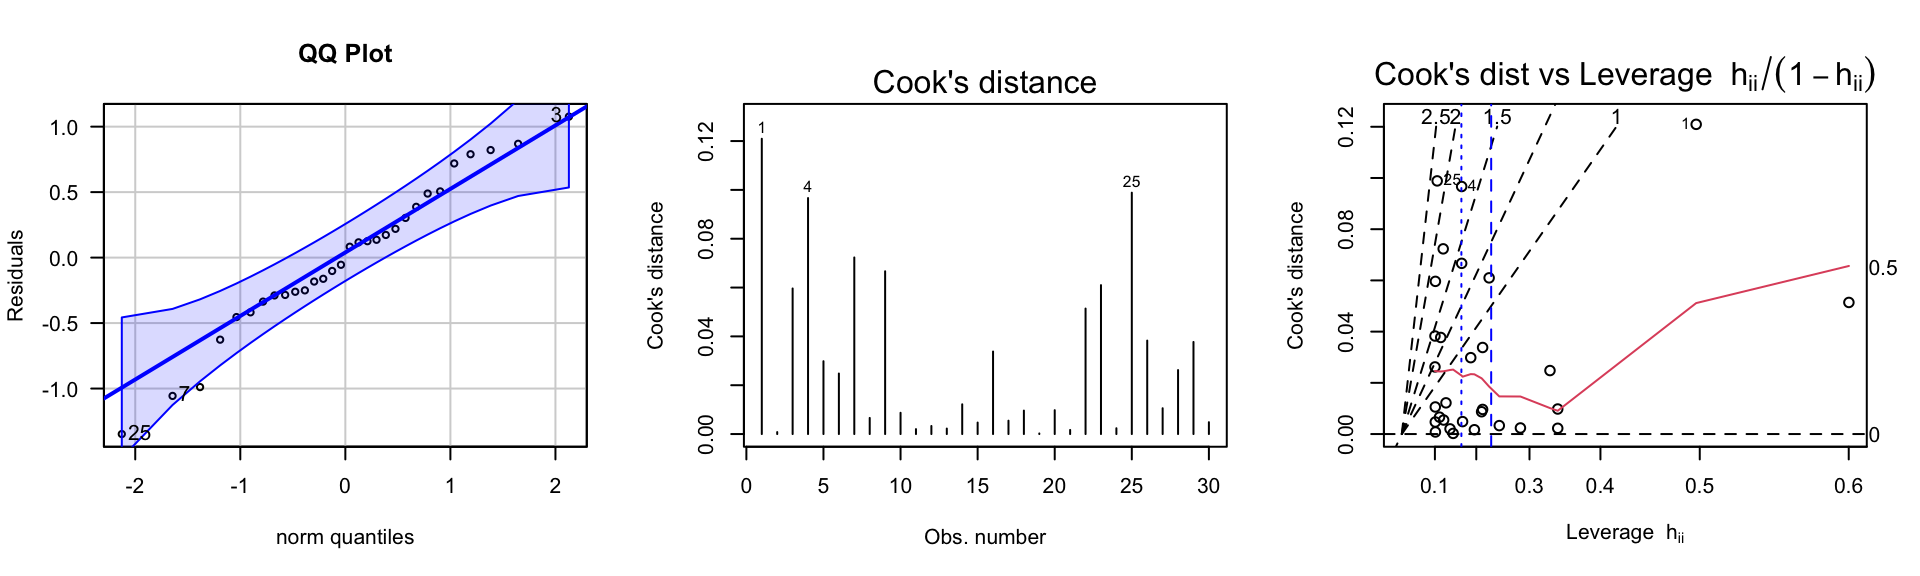
\includegraphics{ADA2_CL_11_ModelEquationsPlots_files/figure-latex/unnamed-chunk-5-1} \end{center}

\hypertarget{ancova-model-faculty-political-tolerances}{%
\section{2. ANCOVA model: Faculty political
tolerances}\label{ancova-model-faculty-political-tolerances}}

A political scientist developed a questionnaire to determine political
tolerance scores for a random sample of faculty members at her
university. She wanted to compare mean scores adjusted for the age for
each of the three categories: full professors (coded 1), associate
professors (coded 2), and assistant professors (coded 3). The data are
given below. Note the higher the score, the more tolerant the
individual.

Below we will fit and interpret a model to assess the dependence of
tolerance score on age and rank. (We will assess model fit in a later
assignment.)

\begin{Shaded}
\begin{Highlighting}[]
\NormalTok{tolerate }\OtherTok{\textless{}{-}}
  \FunctionTok{read\_csv}\NormalTok{(}\StringTok{"\textasciitilde{}/Dropbox/3\_Education/Courses/stat\_528\_ada2/ADA2\_CL\_12\_tolerate.csv"}\NormalTok{) }\SpecialCharTok{\%\textgreater{}\%}
  \FunctionTok{mutate}\NormalTok{(}
    \AttributeTok{rank =} \FunctionTok{factor}\NormalTok{(rank)}
    \CommentTok{\# set "3" as baseline level}
\NormalTok{  , }\AttributeTok{rank =} \FunctionTok{relevel}\NormalTok{(rank, }\StringTok{"3"}\NormalTok{)}
\NormalTok{  )}
\FunctionTok{str}\NormalTok{(tolerate)}
\end{Highlighting}
\end{Shaded}

\begin{verbatim}
spec_tbl_df [30 x 3] (S3: spec_tbl_df/tbl_df/tbl/data.frame)
 $ score: num [1:30] 3.03 4.31 5.09 3.71 5.29 2.7 2.7 4.02 5.52 4.62 ...
 $ age  : num [1:30] 65 47 49 41 40 61 52 45 41 39 ...
 $ rank : Factor w/ 3 levels "3","1","2": 2 2 2 2 2 2 2 2 2 2 ...
 - attr(*, "spec")=
  .. cols(
  ..   score = col_double(),
  ..   age = col_double(),
  ..   rank = col_double()
  .. )
 - attr(*, "problems")=<externalptr> 
\end{verbatim}

\hypertarget{p-write-the-fitted-model-equation.-1}{%
\subsection{\texorpdfstring{\textbf{(3 p)} Write the fitted model
equation.}{(3 p) Write the fitted model equation.}}\label{p-write-the-fitted-model-equation.-1}}

Note in the code what the baseline rank is.

\begin{Shaded}
\begin{Highlighting}[]
\NormalTok{lm\_s\_a\_r\_ar }\OtherTok{\textless{}{-}}
  \FunctionTok{lm}\NormalTok{(}
\NormalTok{    score }\SpecialCharTok{\textasciitilde{}}\NormalTok{ age }\SpecialCharTok{*}\NormalTok{ rank}
\NormalTok{  , }\AttributeTok{data =}\NormalTok{ tolerate}
\NormalTok{  )}
\FunctionTok{summary}\NormalTok{(lm\_s\_a\_r\_ar)}
\end{Highlighting}
\end{Shaded}

\begin{verbatim}
Call:
lm(formula = score ~ age * rank, data = tolerate)

Residuals:
     Min       1Q   Median       3Q      Max 
-1.34746 -0.28793  0.01405  0.36653  1.07669 

Coefficients:
            Estimate Std. Error t value Pr(>|t|)    
(Intercept)  5.42706    0.98483   5.511 1.15e-05 ***
age         -0.01321    0.02948  -0.448   0.6580    
rank1        2.78490    1.51591   1.837   0.0786 .  
rank2       -1.22343    1.50993  -0.810   0.4258    
age:rank1   -0.07247    0.03779  -1.918   0.0671 .  
age:rank2    0.03022    0.04165   0.726   0.4751    
---
Signif. codes:  0 '***' 0.001 '**' 0.01 '*' 0.05 '.' 0.1 ' ' 1

Residual standard error: 0.6378 on 24 degrees of freedom
Multiple R-squared:  0.5112,    Adjusted R-squared:  0.4093 
F-statistic:  5.02 on 5 and 24 DF,  p-value: 0.002748
\end{verbatim}

Use the parameter estimate table above to write out the fitted model
equation. Use indicator function notation for categorical variables. The
equation looks like: \(\hat{y} = [\text{terms}]\).

\hypertarget{solution-3}{%
\subsubsection{Solution}\label{solution-3}}

\[
\widehat{score} = 5.4 
- 0.013 * Age
+ 2.785 * I(\text{rank = 1})
- 1.223 * I(\text{rank = 2})
- 0.072 * Age * I(\text{rank = 1})
+ 0.030 * Age * I(\text{rank = 2})
\]

\hypertarget{p-separate-model-equations.-1}{%
\subsection{\texorpdfstring{\textbf{(2 p)} Separate model
equations.}{(2 p) Separate model equations.}}\label{p-separate-model-equations.-1}}

There's a separate regression line for each faculty rank.

\hypertarget{solution-4}{%
\subsubsection{Solution}\label{solution-4}}

\begin{longtable}[]{@{}lll@{}}
\toprule
Rank & & Fitted Model \\
\midrule
\endhead
1 & &
\(\hat{y}= 5.4 - 0.013 * Age + 2.785 - 0.072 * Age = 8.185 0.085 * Age\) \\
\textbackslash{} & & \\
2 & & \$\hat{y}= 5.4 - 0.013 * Age - 1.223 + 0.030 * Age = 4.177 + 0.017
* Age \$ \\
\textbackslash{} & & \\
3 & & \(\hat{y}= 5.4 - 0.013 * Age\) \\
\bottomrule
\end{longtable}

\hypertarget{p-plot-the-fitted-regression-lines.}{%
\subsection{\texorpdfstring{\textbf{(0 p)} Plot the fitted regression
lines.}{(0 p) Plot the fitted regression lines.}}\label{p-plot-the-fitted-regression-lines.}}

Use symbols/colors/labels to distinguish between the observed and
predicted values and clearly identify the rank. Use the minimum about of
labeling to make it clear. I recommend plotting each line by evaluating
two points then connecting them, for example, by evaluating at age=0 and
age=50.

\hypertarget{solution-5}{%
\subsubsection{Solution}\label{solution-5}}

COVID-19 Year, no hand plotting :(

\begin{center}\includegraphics{ADA2_CL_11_ModelEquationsPlots_files/figure-latex/unnamed-chunk-8-1} \end{center}

\end{document}
